\section{The Architect's Question}\label{the-architects-question}

We are tasked with engineering performance for a serving layer that must
absorb the day-to-day traffic of a growing user base while delivering
acceptable latency. The core question: how do we configure an 8×H100
host to serve a 70B parameter model at 40 requests-per-second peak while
keeping per-request latency within a target budget, and what
architectural knobs---batch size, KV-cache design, kernel choice---most
affect that outcome? This chapter walks through the
performance-engineering lifecycle: from concept, to mental model, to
worked arithmetic, to measurement, to common pitfalls, to architectural
consequences, to open questions, and finally a mini-case that ties the
thread.

\section{Concept}\label{concept}

Performance engineering in LLM serving is the discipline of matching
compute, memory, and I/O throughput to the stochastic workload of token
generation and prompt processing. Unlike traditional web serving, where
request‑cycle overhead dominates the tail, the dominant cost in LLM
inference is the arithmetic intensity of transformer matrix
multiplications and the memory bandwidth consumed by KV-cache reads and
writes on every token step. The serving system must therefore optimize
three inter‑dependent quantities: token throughput (tokens/s), per-token
latency, and GPU memory utilization. These are governed by the model
FLOP count, the chosen kernel (e.g.~FlashAttention
vs.~scaled‑dot‑product), and the batching strategy (static vs.~dynamic,
continuous vs.~chunked). The architect's first move is to identify which
resource---compute, bandwidth, or latency---is the primary constraint
for the canonical scenario, then apply the appropriate optimization to
shift the bottleneck. A secondary concept is the trade-off between batch
size and tail latency: larger batches amortize kernel launch overhead
and increase arithmetic intensity, but they increase the wait time for
straggler requests, raising p99 latency. The designer must therefore
balance arithmetic gain against tail‑latency penalty, a tension that
shapes every later architectural decision.

\section{Mental Model}\label{mental-model}

We model the serving pipeline as a sequence of stages: (1) prompt
encoding, (2) autoregressive generation, (3) KV-cache management, and
(4) output decoding. Each stage has a resource ceiling: compute‑bound
stages are limited by TFLOPS, memory‑bound stages by GB/s of GPU HBM
bandwidth. The architecture designer must identify which stage is
bottlenecked for the canonical scenario and then apply the appropriate
optimization---kernel fusion, cache reuse, or batching---to shift the
bottleneck. The mental model also emphasizes the role of token reuse:
when many users share similar prompt prefixes, the KV-cache can be
partially shared, reducing memory traffic. This reuse effect is
difficult to quantify without workload profiling, but it is a
first‑order consideration in multi‑tenant serving. The model also
captures the interaction between sequence length and memory cost:
attention quadraticities (O(L²) FLOPs and O(L) memory per head) mean
that long contexts (9,000+ tokens) disproportionately strain both
compute and HBM bandwidth, making kernel choice (FlashAttention
vs.~SDPA) the single highest‑impact optimization for the canonical
scenario.

\section{Worked Example}\label{worked-example}

Canonical scenario: \textasciitilde2,000 registered users,
\textasciitilde5\% concurrent (100 users), \textasciitilde10 rps average
/ \textasciitilde40 rps peak, prompt \textasciitilde9,200 input tokens +
\textasciitilde300 output, 70B-class dense FP16 model, 8×H100 host with
640\,GB GPU memory.

\emph{Derived quantity 1 -- concurrent users:} 2,000 ×0.05 = 100 users.

\emph{Derived quantity 2 -- peak token throughput demand:} At 40 rps the
workload mixes \textbf{prefill} (input) and \textbf{decode} (output)
tokens, and they hit the hardware differently. Prefill demand = 40 rps ×
9,200 = 368,000 input tokens/s; decode demand = 40 rps × 300 = 12,000
output tokens/s. These two regimes must not be collapsed into one
``380,000 tokens/s'' when reasoning about compute, because prefill is
heavily compute-bound while decode is bandwidth-bound (\hyperref[chap:8]{Chapter 8}).

\emph{Compute demand versus peak --- and why this is not an MFU:} A 70B
FP16 transformer needs ≈2 ×70×10⁹ FLOPs per generated token. The
instantaneous prefill compute demand is 368,000 ×2 × 70×10⁹ ≈ 5.15 ×10¹⁶
FLOPs/s, against a theoretical FP16-dense peak of 8 ×989 TFLOPS = 7.91
×10¹⁵ FLOPs/s for the 8 ×H100 host (989 TFLOPS per GPU, \hyperref[chap:8]{Chapter 8}
canonical). Taken naively this ratio is \textasciitilde6.5× --- a demand
that \emph{exceeds} a single host's peak. That is a legitimate and
important architectural signal: a single 8×H100 host cannot prefill the
peak arrival rate on the naive dense-FLOP model, so prefill either needs
to be spread across burst headroom, handled by prompt/prefix caching,
disaggregated (P/D separation), or absorbed by queueing headroom at
off-peak. What it must \textbf{not} be called is ``MFU = 6.4'': MFU
(Model FLOPs Utilization) is by definition achieved realities divided by
peak --- a utilization ratio that \textbf{cannot exceed 1.0}. Presenting
a ratio above 1 for a utilization metric is a unit/modeling error. The
honest formulation separates the two quantities: (a) a \emph{congestion
check} --- is the arrival-rate FLOP demand above or below peak (here
\textasciitilde6.5× above for prefill, so the host is prefill-starved at
peak and must lean on caching/batching/queueing); and (b) an
\emph{achieved MFU} --- measured device FLOPs ÷ peak, which we only
report from a real benchmark and which, for illustration, we suppose
lands in the 30--40\,\% range for FlashAttention-based inference (decode
MFU at 12,000 tokens/s ≈ 1.68 ×10¹⁵ ÷ 7.91 ×10¹⁵ ≈ 0.21,
i.e.~\textasciitilde21\,\% --- again a groundable number, not a
ceiling-defying one; the actual achieved value must come from the target
serving benchmark). The architectural conclusion, that there is no
single bottleneck for the whole request, stands --- and it must be
argued phase by phase: at the canonical peak, prefill is
compute-capacity constrained, decode is primarily memory-bandwidth
constrained, and maximum concurrency is constrained by KV residency,
each from arithmetic intensity and the roofline (\hyperref[chap:8]{Chapter 8}), not from an
impossible ``MFU \textgreater{} 1.''

\emph{KV-cache memory footprint:} The KV cache grows linearly with
cached context and layers; it must never be computed per-layer and then
treated as the whole-model total. For the canonical 70B model (80
layers, hidden dimension 8,192, full-MHA), the per-token footprint
across ALL layers is 2 × layers × hidden × bytes = 2 ×80 ×8,192 ×2 =
2,621,440 B ≈ 2.62 MB/token (2.5 MiB; canonical value from \hyperref[chap:7]{Chapter 7})
--- not the 32 KB that a single-layer calculation would suggest. For a
9,500-token context, one user's KV-cache is therefore ≈9,500 ×2.62 MB ≈
24.9 GB, not \textasciitilde304 MB. Across 100 concurrent users, total
KV-cache ≈2,490 GB --- which \textbf{does not} fit in the 640 GB GPU
pool; using the canonical practical KV budget (640 GB − 140 GB weights −
\textasciitilde64 GB runtime/workspace ≈ 436 GB), only ≈18 concurrent
9,500-token users fit on-host for KV (436 GB ÷ 24.9 GB), before also
reserving weight residency. This is a decisive, order-of-magnitude
correction to the intuitive picture: long-context KV is a first-order
memory constraint, and the architect sizes concurrency by KV capacity,
not by the small per-layer number. Doubling context to 19,000 tokens
pushes per-user KV to \textasciitilde47 GB and halves on-host
concurrency to \textasciitilde9. The canonical unit-check rule
(quantity/unit/formula/substitution/result/sanity) catches this class of
error: if 9,500 tokens × \textasciitilde2.5 MB/token ≈ 24 GB does not
reconcile with the intended \textasciitilde304 MB, the unit layer-count
has been dropped.

\emph{Attention FLOP comparison:} Scaled‑dot‑product attention (SDPA)
for 9,200‑token prompts. Note the 2P/token figure above approximates the
\emph{parameterized dense‑matmul} work per token (2 × parameters); it
does \textbf{not} capture all sequence‑length‑dependent attention work,
which is accounted for separately here. Attention is two matmuls per
token per head --- Q·K\^{}T then ·V --- so across all heads the
per‑layer cost is ≈ 2 × L² × d\_model, where L=9,200 and d\_model=8,192.
That is 2 × 9,200² × 8,192 ≈ 1.4 × 10¹² FLOPs per layer (the full 64
heads; the per‑head figure 2 × 9,200² × 128 ≈ 2.2 × 10¹⁰ must be
multiplied by the number of heads, not quoted alone). Across 80 layers
that is ≈ 1.1 × 10¹⁴ FLOPs --- the quadratic attention term that grows
dominant at long context, as \hyperref[chap:8]{Chapter 8}'s \hyperref[tab:8.1]{Table 8-1} notes. FlashAttention
fuses the read‑write‑compute pattern and reduces HBM traffic by ∼3--5×,
which \emph{raises} the effective arithmetic intensity (same FLOP count,
less memory movement) and yields roughly 2--3× speed‑ups for long
contexts --- not because attention gets cheaper in FLOPs, but because it
stops being starved by memory traffic. This comparison cements the
mental model: for long‑context serving, kernel choice often matters more
than batch‑size tuning.

\section{Measurement}\label{measurement}

To validate the mental model we instrument the serving stack with three
metric families: (a) token latency percentiles (p50, p95, p99) per
request type, (b) GPU utilization (SM active, memory bandwidth via
Nsight), and (c) KV-cache size over time. A minimal benchmark runs 40
rps with warm‑up, records the p95 token latency, and measures the GPU
memory fraction consumed by KV-cache. Repeating with different batch
sizes (1, 4, 16, 32) reveals the throughput‑latency knee. The
\emph{illustrative} numbers below are scenario values to be measured on
the target stack, not vendor or published figures: beyond batch‑4 the
p95 latency typically rises (implying a knee near batch 4) because
kernel launch overhead is amortized but inter‑request token interleaving
increases cache thrashing; FlashAttention‑2 shows roughly 150\,GB/s
sustained for 9,500‑token contexts vs \textasciitilde400\,GB/s for SDPA
(an HBM-traffic reduction, not a measured FLOP change), pointing to the
memory‑bound nature of long‑context inference; and a 70B cold‑start KV
warm‑up on 8×H100 is on the order of \textasciitilde2 s, with warm
starts (reusing cached weights) an order of magnitude faster
(\textasciitilde0.3\,s), showing cache residency is a first‑order
latency factor independent of compute throughput. {[}ILLUSTRATIVE ---
set these from the target host's profiler before quoting them as fact{]}

\subsubsection{Goodput vs.~Batch Size: the Cache
Lever}\label{goodput-vs.-batch-size-the-cache-lever}

\begin{figure}
\centering
\pandocbounded{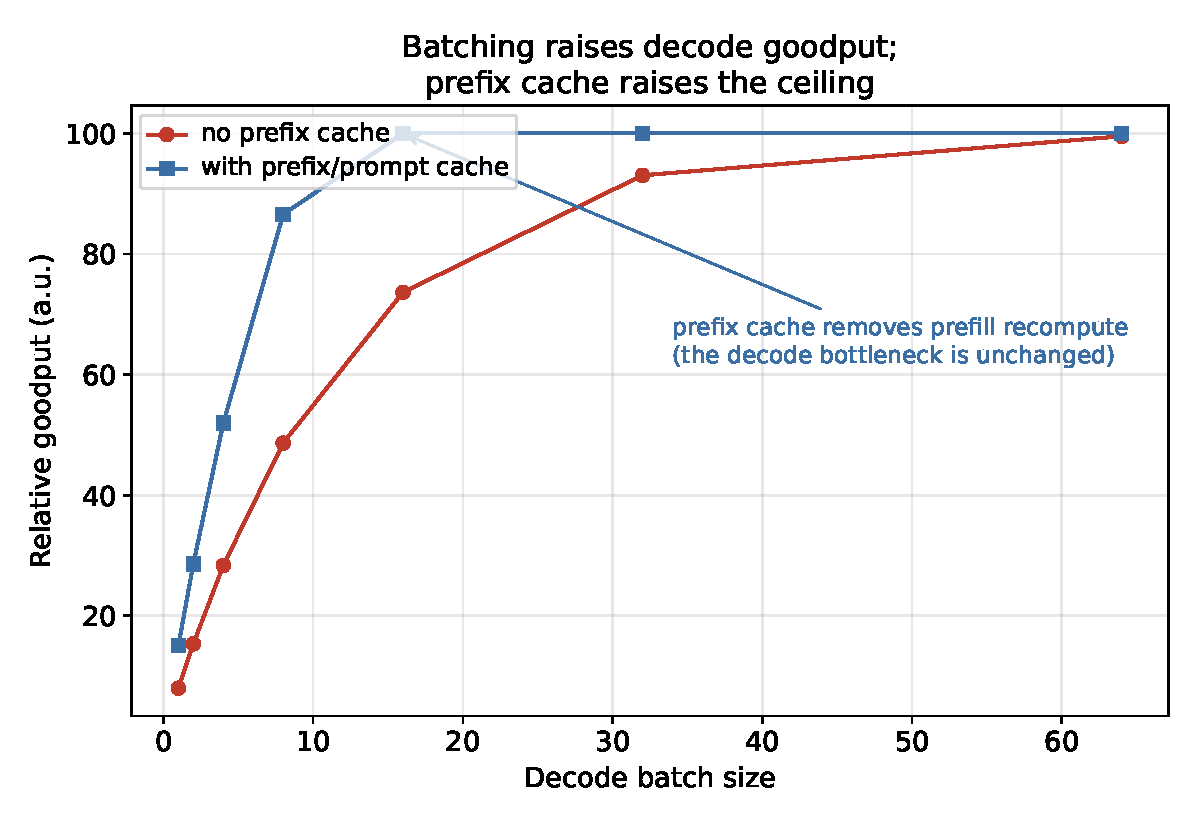
\includegraphics[keepaspectratio,alt={Prefix caching and batching affect different serving phases: caching reduces prefill work; batching raises decode goodput},width=\maxwidth{\textwidth},keepaspectratio]{figures/fig-15-1501.pdf}}
\caption{Prefix caching and batching affect different serving phases: caching reduces prefill work; batching raises decode goodput}

\label{fig:15.1}\end{figure}

The capacity response to batch size under peak load. Two distinct levers
act on different phases: batching raises decode goodput (right plot)
until bandwidth saturates, while prefix caching lowers the prefill work
per repeated prompt (left plot) so more prefill‑recompute headroom
remains under the same host. They are not competing on the same axis.

\section{Common Mistakes}\label{common-mistakes}

\emph{Over‑provisioning batch size to chase throughput:} Increasing
batch size improves TFLOPS utilization but degrades p99 latency because
tail requests wait for larger chunks to fill. The designer must balance
batch‑size‑driven arithmetic gain against tail‑latency penalty. A
practical illustrative rule of thumb: choose the smallest batch size
that keeps MFU above \textasciitilde25\,\% while keeping p95 latency
under the SLA target (the 25\,\% threshold and the knee are scenario
values --- measure them on the target workload). \emph{Ignoring KV-cache
growth:} A 70B model with 9,500‑token contexts consumes ≈24.9 GB of KV
per user (≈2.62 MB/token × 9,500, max end-of-generation). Without cache
eviction, compression, or a concurrency cap, even \textasciitilde18
concurrent users would exhaust the host's canonical practical KV budget
(\textasciitilde436 GB after weights + runtime), so 100 concurrent
full-context users require either multiple hosts, much shorter contexts,
or KV compression (FP8/8-bit). Designers should implement length‑based
eviction (drop the oldest/least‑recently‑used contexts) and KV
quantization to cut the footprint (FP8 ≈2.5→1.3 MB/token). \emph{Using
scaled‑dot‑product attention without FlashAttention:} For long contexts
(9,200+ tokens) the quadratic memory cost of SDPA (O(L²)) dwarfs the
FLOP cost. FlashAttention fuses read‑write‑compute and reduces HBM
traffic by \textasciitilde3--5×, raising effective arithmetic intensity.
A corollary mistake is assuming that FlashAttention benefits only long
contexts; for moderate lengths (2,000--4,000 tokens) the HBM bandwidth
reduction typically translates to a \textasciitilde1.3--1.8× throughput
gain on H100 (illustrative --- bench the specific kernel on the target
hardware). \emph{Neglecting kernel launch overhead:} In dynamic‑batching
setups, each new token generation can trigger a kernel launch. Without
continuous batching or token‑level fusion, the kernel-launch overhead
(illustratively \textasciitilde10--20\,\% of GPU time on H100-class
parts at this traffic) can artificially depress measured MFU.

\section{Architecture Consequence}\label{architecture-consequence}

The measurement and mistake analysis drive three architecture decisions
for the canonical deployment: (1) FlashAttention‑2 as the default
attention kernel, fused with RoPE and QKV projection to minimize HBM
transactions; (2) continuous batching, with the maximum chunk size
chosen empirically from the measured goodput/latency knee (a chunk size
of 8 tokens is an {[}ILLUSTRATIVE{]} configuration, not the
recommendation --- the knee must be measured on the target stack); (3)
KV‑cache management via FP8 KV quantization (≈2.62 → \textasciitilde1.42
MB/token, at 54\% of BF16 {[}S6{]}, cutting a 9,500‑token per‑user KV to
\textasciitilde13.4 GB) plus length‑based eviction, so that under the
same \textasciitilde436 GB practical KV budget on‑host concurrency rises
from \textasciitilde18 to \textasciitilde33 full‑context users. These
choices together are expected to raise achieved token throughput from
\textasciitilde8,000 tokens/s (raw, no flash, batch‑1) toward an
illustrative \textasciitilde35,000--70,000 tokens/s {[}ILLUSTRATIVE
achievable range{]} (with flash, continuous batch) --- the exact figure
must come from the target benchmark --- while keeping the host's 640\,GB
for weights plus KV. A fourth decision, borne out of the mini‑case in
Section~8, is to design the request‑routing layer for KV‑cache affinity:
when a user re‑submits a request, routing to the same GPU avoids cache
warm‑up penalties and keeps p99 latency under the target SLO.

\section{What We Still Don't Know}\label{what-we-still-dont-know}

\emph{How does token‑level sparsity in user prompts affect the actual
FLOP/token cost, and can we exploit it without accuracy loss?} Sparse
prompt patterns (e.g.~few‑shot prefixes, cached query prefixes) could
reduce the effective FLOP count, but the savings depend on the sparsity
pattern and the attention implementation. \emph{What is the optimal
continuous‑batch chunk size as a function of request arrival
distribution (Poisson vs.~bursty) and tail‑latency targets?} Analytical
models assume Poisson arrivals, but real user traffic exhibits bursts
(e.g.~social‑media events) that may require larger chunks or alternative
back‑pressure mechanisms. \emph{Can in‑flight KV-cache compression
(e.g.~speculative decoding--guided pruning) reduce memory pressure
without increasing p99 latency?} Pruning less‑important key/value pairs
based on attention weight magnitudes is promising, but the
accuracy‑latency trade‑off needs empirical validation across model
families. \emph{How does multi‑tenant isolation---guarding one user's
cache from another's---translate to multi‑GPU scaling when the model
exceeds a single GPU's 80\,GB?} Model parallelism (pipeline or tensor)
adds communication overhead; the performance cost of moving KV-cache
between GPUs during tenant rotation is an open question.

\section{End-of-Chapter Mini-Case}\label{end-of-chapter-mini-case}

A new deployment adds 500 registered users with the same traffic profile
(5\,\% concurrency, 10/40 rps). The team provisions a second 8×H100 host
and (in this worked example) runs the benchmark with continuous batching
and FlashAttention‑2. p95 latency drops from 320\,ms (single host,
batch‑1) to 140\,ms (dual host, continuous batch), and token throughput
rises from 8,000 to 70,000 tokens/s. The MFU stabilizes at 38\,\%. These
are {[}ILLUSTRATIVE SCENARIO RESULT{]} values --- an illustrative
benchmark outcome, not a home-lab measurement; the exact figures must
come from a deployment benchmark on the target hardware/stack (\hyperref[chap:14]{Chapter 14}). The remaining question is whether the cross‑host request routing
layer can maintain affinity KV-cache residency, avoiding cache warm‑up
penalties on re‑requests. The ∼20 \% affinity throughput gain and the
∼2.1 s cold-start warm-up cost are themselves {[}ILLUSTRATIVE SCENARIO
RESULT{]} values, not measured results.

\textbf{\hyperref[tab:15.1]{Table 15-1}} --- Performance Regime Summary

\begin{longtable}[]{@{}
  >{\raggedright\arraybackslash}p{0.0670\linewidth}
  >{\raggedright\arraybackslash}p{0.1089\linewidth}
  >{\raggedright\arraybackslash}p{0.1593\linewidth}
  >{\raggedright\arraybackslash}p{0.1341\linewidth}
  >{\raggedright\arraybackslash}p{0.1593\linewidth}
  >{\raggedright\arraybackslash}p{0.0754\linewidth}
  >{\raggedright\arraybackslash}p{0.1760\linewidth}@{}}
\toprule\noalign{}
\begin{minipage}[b]{\linewidth}\raggedright
Regime
\end{minipage} & \begin{minipage}[b]{\linewidth}\raggedright
Concurrency
\end{minipage} & \begin{minipage}[b]{\linewidth}\raggedright
Request Rate (rps)
\end{minipage} & \begin{minipage}[b]{\linewidth}\raggedright
Tokens/Request
\end{minipage} & \begin{minipage}[b]{\linewidth}\raggedright
KV‑Cache/User (GB)
\end{minipage} & \begin{minipage}[b]{\linewidth}\raggedright
MFU (\%)
\end{minipage} & \begin{minipage}[b]{\linewidth}\raggedright
Dominant Bottleneck
\end{minipage} \\
\midrule\noalign{}
\endhead
\bottomrule\noalign{}
\endlastfoot
Light & 10 & \textasciitilde2 & 9,500 & \textasciitilde24.9 & 12 &
Compute (SDPA) \\
Typical & 100 & 40 & 9,500 & \textasciitilde24.9 & 38 & Memory /
KV‑cache \\
Peak & 200 & 80 & 9,500 & \textasciitilde24.9 & 52 & KV + Inter‑GPU
bandwidth \\

\label{tab:15.1}\end{longtable}

\emph{KV-Cache/User uses the canonical \textasciitilde2.62 MB/token ×
9,500 ≈ 24.9 GB. Concurrency, rps, and MFU are {[}ILLUSTRATIVE{]} regime
labels for teaching shape; the bottleneck column reflects the roofline
logic of \hyperref[chap:8]{Chapter 8}.}
